\documentclass{ximera}

\outcome{Find the intervals where a function is increasing or decreasing.}
\outcome{Find the intervals where a function is concave up or down.}
\outcome{Find any asymptotic behaviors a function may have: vertical, horizontal, or slant.}
\outcome{Determine how the graph of a function looks without using a calculator.}

\author{Nela Lakos \and Kyle Parsons}
\begin{document}
\begin{exercise}
Consider the $f$ given by
\[
f(x) = \frac{x}{\sqrt{x^2-9}}.
\]

The domain of $f$ (written from left to right) is $\left(\answer{-\infty},\answer{-3}\right)\cup\left(\answer{3},\answer{\infty}\right)$.

$f$ has horizontal asymptotes (from bottom to top) at $y=\answer{-1}$ and $y=\answer{1}$.

$f$ has vertical asymptotes (from left to right) at $x=\answer{-3}$ and $x=\answer{3}$.

The derivative of $f(x)$ is
\[
f'(x) =\frac{ \answer{-9}}{(x^2-9)^{3/2}}.
\]

The second derivative of $f(x)$ is
\[
f''(x) =\frac{\answer{27x}}{(x^2-9)^{5/2}}.
\]

On the interval $(-\infty,-3)$ $f$ is \wordChoice{\choice{increasing}\choice[correct]{decreasing}\choice{not defined}} and \wordChoice{\choice{concave up}\choice[correct]{concave down}\choice{not defined}}.

On the interval $(-3,3)$ $f$ is \wordChoice{\choice{increasing}\choice{decreasing}\choice[correct]{not defined}} and \wordChoice{\choice{concave up}\choice{concave down}\choice[correct]{not defined}}.

On the interval $(3,\infty)$ $f$ is \wordChoice{\choice{increasing}\choice[correct]{decreasing}\choice{not defined}} and \wordChoice{\choice[correct]{concave up}\choice{concave down}\choice{not defined}}.

Consider the graphs below.

\begin{center}
  \resizebox{.3\textwidth}{!}{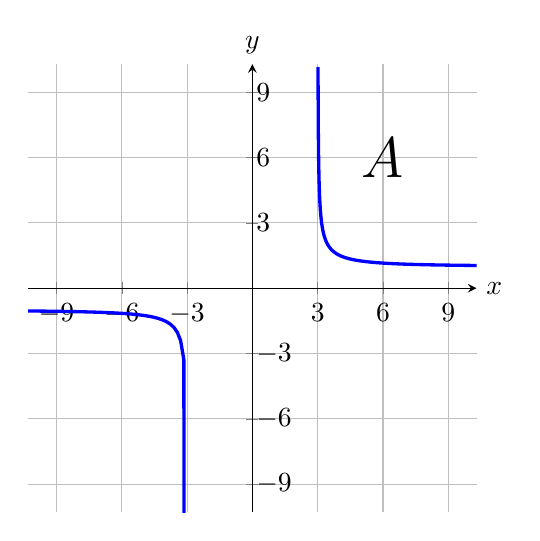
\begin{tikzpicture}
    \begin{axis}[
        xmin=-10.3,xmax=10.3,ymin=-10.3,ymax=10.3,
        clip=true,
        unit vector ratio*=1 1 1,
        axis lines=center,
        grid = major,
        ytick={-21,-18,...,21},
    	xtick={-21,-18,...,21},
        xlabel=$x$, ylabel=$y$,
        y tick label style={anchor=west},
        every axis y label/.style={at=(current axis.above origin),anchor=south},
        every axis x label/.style={at=(current axis.right of origin),anchor=west},
      ]
      \addplot[very thick,blue,domain=-10.3:-3,samples=50] plot{x/sqrt(x^2-9)};
      \addplot[very thick,blue,domain=3:10.3,samples=500]  plot{x/sqrt(x^2-9)};

      \node at (axis cs:6,6) {\huge$A$};
      \end{axis}`
  \end{tikzpicture}}
  \resizebox{.3\textwidth}{!}{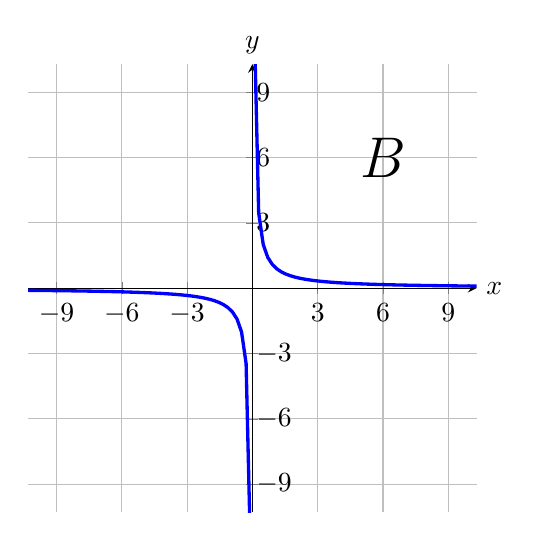
\begin{tikzpicture}
    \begin{axis}[
        xmin=-10.3,xmax=10.3,ymin=-10.3,ymax=10.3,
        clip=true,
        unit vector ratio*=1 1 1,
        axis lines=center,
        grid = major,
        ytick={-21,-18,...,21},
    	xtick={-21,-18,...,21},
        xlabel=$x$, ylabel=$y$,
        y tick label style={anchor=west},
        every axis y label/.style={at=(current axis.above origin),anchor=south},
        every axis x label/.style={at=(current axis.right of origin),anchor=west},
      ]
      \addplot[very thick,blue,domain=-10.3:-0.08,samples=50] plot{1/x};
      \addplot[very thick,blue,domain=0.08:10.3,samples=50] plot{1/x};

      \node at (axis cs:6,6) {\huge$B$};
      \end{axis}
  \end{tikzpicture}}
  \\
  \resizebox{.3\textwidth}{!}{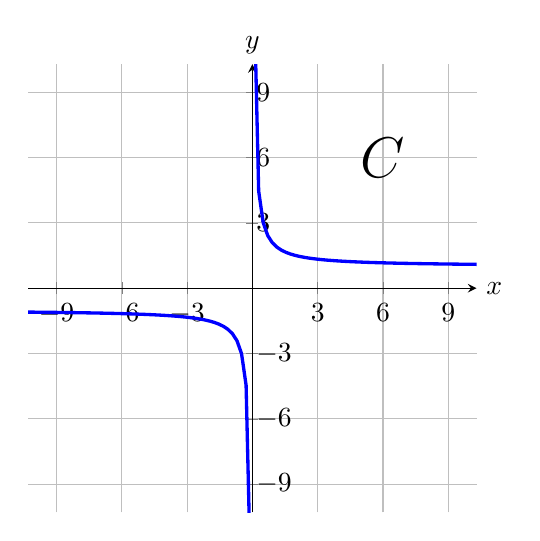
\begin{tikzpicture}
    \begin{axis}[
        xmin=-10.3,xmax=10.3,ymin=-10.3,ymax=10.3,
        clip=true,
        unit vector ratio*=1 1 1,
        axis lines=center,
        grid = major,
        ytick={-21,-18,...,21},
    	xtick={-21,-18,...,21},
        xlabel=$x$, ylabel=$y$,
        y tick label style={anchor=west},
        every axis y label/.style={at=(current axis.above origin),anchor=south},
        every axis x label/.style={at=(current axis.right of origin),anchor=west},
      ]
      \addplot[very thick,blue,domain=-10.3:-0.08,samples=50] plot{1/x-1};
      \addplot[very thick,blue,domain=0.08:10.3,samples=50] plot{1/x+1};
      
      \node at (axis cs:6,6) {\huge$C$};
      \end{axis}
  \end{tikzpicture}}
  \resizebox{.3\textwidth}{!}{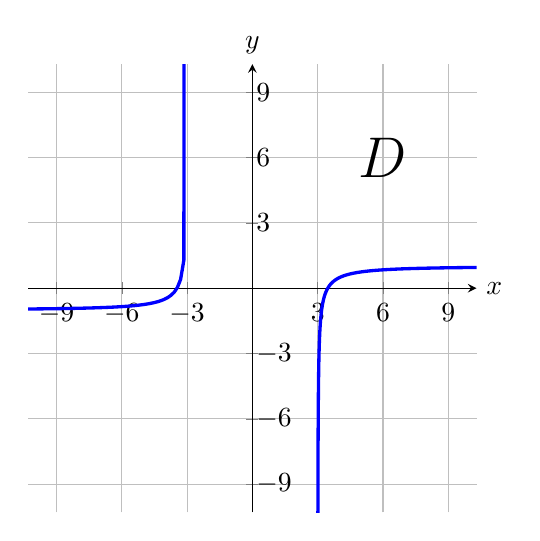
\begin{tikzpicture}
    \begin{axis}[
        xmin=-10.3,xmax=10.3,ymin=-10.3,ymax=10.3,
        clip=true,
        unit vector ratio*=1 1 1,
        axis lines=center,
        grid = major,
        ytick={-21,-18,...,20},
    	xtick={-21,-18,...,20},
        xlabel=$x$, ylabel=$y$,
        y tick label style={anchor=west},
        every axis y label/.style={at=(current axis.above origin),anchor=south},
        every axis x label/.style={at=(current axis.right of origin),anchor=west},
      ]
      \addplot[very thick,blue,domain=-10.3:-3,samples=50] plot{-x/sqrt(x^2-9)-2};
      \addplot[very thick,blue,domain=3:10.3,samples=800]  plot{-x/sqrt(x^2-9)+2};
      
      \node at (axis cs:6,6) {\huge$D$};
      \end{axis}
  \end{tikzpicture}}
\end{center}
  
Which graph correctly depicts $f$?
\begin{multipleChoice}
\choice[correct]{$A$}
\choice{$B$}
\choice{$C$}
\choice{$D$}
\end{multipleChoice}

$f$ \wordChoice{\choice[correct]{is}\choice{is not}} one-to-one.

The inverse of $f(x)$ is
\[
f^{-1}(x) = \answer{\frac{3x}{\sqrt{x^2-1}}}.
\]

The domain of $f^{-1}(x)$ (from left to right) is $\left(\answer{-\infty},\answer{-1}\right)\cup\left(\answer{1},\answer{\infty}\right)$.



\end{exercise}
\end{document}
